\section{节标题}
\label{xdtz}

这是正文这是正文这是正文这是正文这是正文这是正文这是正文这是正文。\textcolor{myblue}{\textbf{相对突出。}}\snote{这是旁注。这里的相对指的是 XX}这是正文这是正文这是正文。这是正文这是正文这是正文。这是正文这是正文这是正文。

\subsection{小节标题}
\label{computer}



%\textcolor{myblue}{\textbf{1. 用机器解放重复计算的双手 } }
\subsubsection{\textcolor{myblue}{\textbf{1. 小标题 }}}
1231231231231i哦Sharpe文化


\begin{figure}[H]
	\begin{center}
		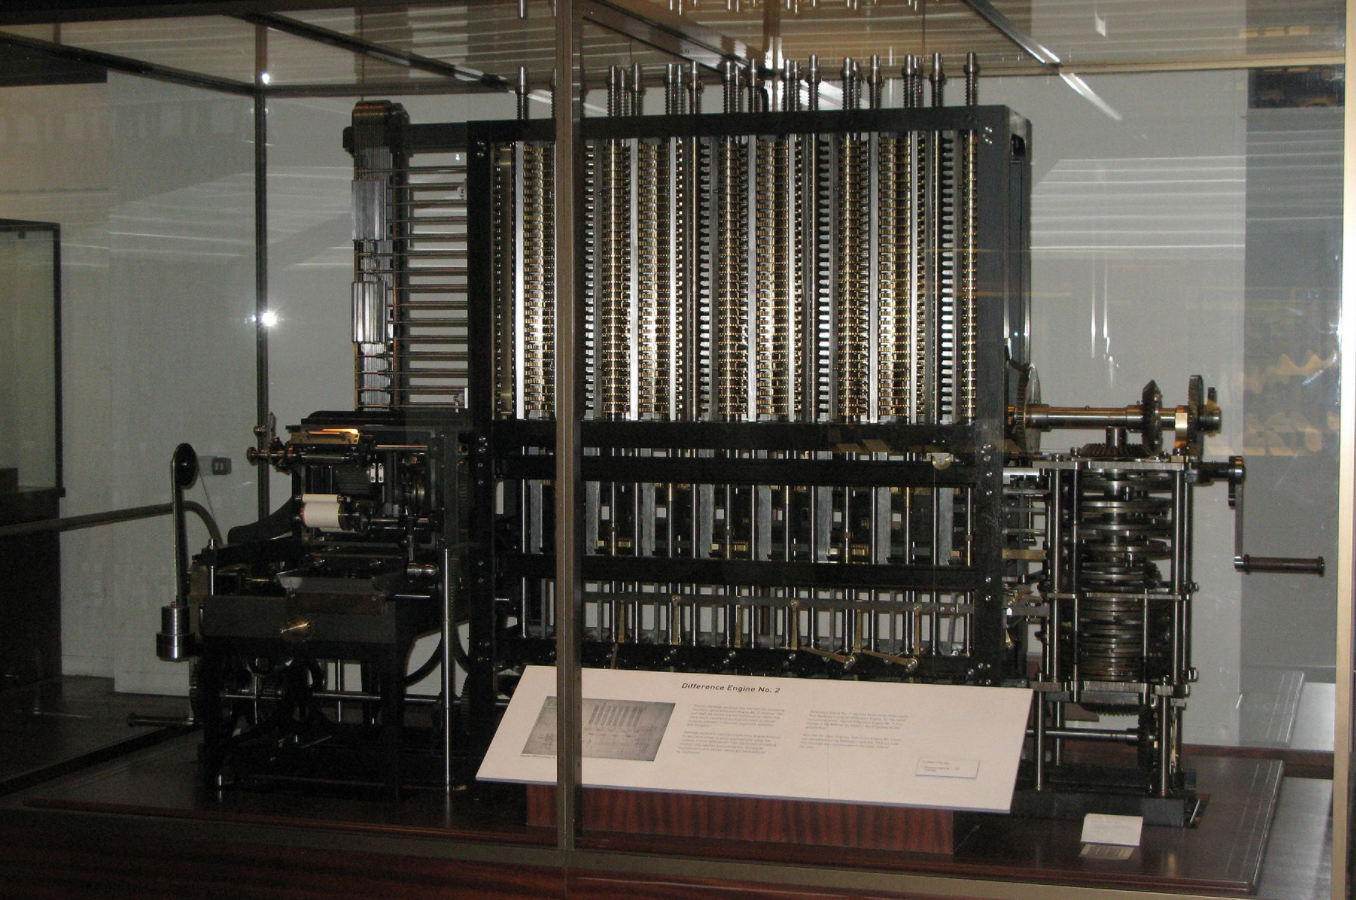
\includegraphics[width=0.6\columnwidth]{Chapter1/graph/差分机2号.png} \\
	\end{center}
	\vspace{-10pt}
	\caption{差分机2号} \label{fig:fenxiji}
	\vspace{-10pt}
\end{figure}

















